\documentclass[english,serif,mathserif,usenames,dvipsnames]{beamer}
\usetheme[informal]{gc3}

\usepackage[T1]{fontenc}
\usepackage[utf8]{inputenc}
\usepackage{babel}

\usepackage{fancyvrb}
%% This is optional: it adds a few commands and environment we
%% regularly use in our slide sets
\usepackage{gc3}

\lstnewenvironment{stdout}{%
  \lstset{language=sh,basicstyle=\tiny\ttfamily\bfseries,escapechar=^}
}{}%


\begin{document}

%% Optional Argument in [Brackets]: Short Title for Footline
\title[GC3Pie Tools]{An Introduction to GC3Pie Session-based scripts}
\author{Riccardo Murri \texttt{<riccardo.murri@gmail.com>}}
\date{\today}

%% Makes the title slide
\maketitle

% # Agenda (1/3)
%
% 1. Introduction
%    * What is GC3Pie?

\begin{frame}
  \frametitle{What is GC3Pie?}
  GC3Pie is \ldots
  \begin{enumerate}
  \item An \emph{opinionated} Python framework for defining and running computational workflows;
  \item \alert<2>{A \emph{rapid development toolkit} for running user applications on clusters and IaaS cloud resources;}
  \item The worst name ever given to a middleware piece\ldots
  \end{enumerate}

  \+
  \uncover<2>{%
    As \emph{users}, \alert<2>{you're mostly interested in this part.}
  }%
\end{frame}


\begin{frame}
  \frametitle{Who am I?}
  \begin{center}
    Systems administrator and programmer.
    \\ \+
    At UZH since 2010, first at GC3 then at S3IT.
    \\ \+
    Developer of GC3Pie since 2010.
  \end{center}
\end{frame}


\begin{frame}
  \begin{center}
    {\Huge and what about you?}
  \end{center}
\end{frame}


\begin{frame}
  \frametitle{Outline of this training, 1}
  \begin{enumerate}
  \item Concepts and glossary
  \item Usage of a session-based script
  \item Command-line tools mainly useful for debugging
  \end{enumerate}
\end{frame}


\begin{frame}
  \frametitle{Outline of this training, 2}
  \begin{center}
    We'd like the training to be \\ as interactive and informal as possible.

    \+ If you have a question, just ask -- don't wait.
  \end{center}
\end{frame}


% chapter division
\section{Concepts and glossary}
\part{Concepts and glossary}

\begin{frame}
  \frametitle{What is GC3Pie?}
  GC3Pie is \ldots
  \begin{enumerate}
  \item \alert<2>{An \emph{opinionated} Python framework for defining and running computational workflows;}
  \item \alert<1>{A \emph{rapid development toolkit} for running user applications on clusters and IaaS cloud resources;}
  \item The worst name ever given to a middleware piece\ldots
  \end{enumerate}

  \+
  \only<1>{As \emph{users}, \alert<1>{you're mostly interested in this part.}}
  \only<2>{\small However, you need to understand the basic concepts ;-)}
\end{frame}


\begin{frame}
  \frametitle{A typical GC3Pie script?}

\begin{semiverbatim}
    > ./warholize.py uzh-logo.png --watch 1
\end{semiverbatim}

  \begin{tabular}[c]{ccc}
    \includegraphics[width=0.4\textwidth]{fig/uzh-logo.png}
    &
    
\includegraphics[width=0.1\textwidth]{fig/arrow.pdf}
    &
    \includegraphics[width=0.4\textwidth]{fig/warholized-uzh-logo.png}
  \end{tabular}
\end{frame}


\begin{frame}
  \frametitle{How does ``Warholize'' work?}

  \begin{center}
    It is a GC3Pie \emph{workflow}: each box is a distinct application
    instance that is run.

    \+
    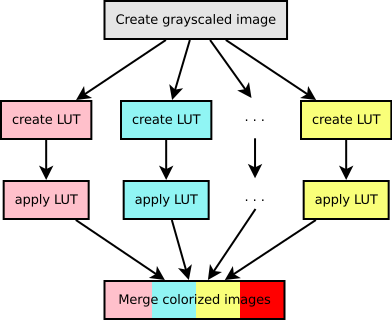
\includegraphics[width=0.70\textwidth]{fig/warholize-wkf}
  \end{center}
\end{frame}


\begin{frame}
  \frametitle{What GC3Pie handles for you}

  \begin{enumerate}\small
  \item Resource allocation (e.g. starting new instances on
    ScienceCloud)
  \item Selection of resources for each application in the session
  \item Data transfer (e.g. copying input files in the new instances)
  \item Remote execution of the application
  \item Retrieval of results (e.g. copying output files from the
    running instance)
  \item De-allocation of resources
  \end{enumerate}

\end{frame}


% 2. Concepts and glossary
%    * Task / Application / Run

\begin{frame}
  \frametitle{GC3Pie glossary: Application}
  \begin{quote}
    GC3Pie runs \alert<2-3>{user applications}
    \\
    on clusters and IaaS cloud resources
  \end{quote}

  \uncover<2-3>{
    \+ \alert<2>{An \texttt{Application} is just a command to execute.}

    \+
    \only<2>{If you can run it in the terminal, \\ you can run it in GC3Pie.}
    \only<3>{
      \alert<3>{A single execution of an \texttt{Application} \\ is indeed called a \texttt{Run}.}

      \+ (Other systems might call this a ``Job''.)
    }
  }
\end{frame}



\begin{frame}
  \frametitle{GC3Pie glossary: Task}
  \begin{quote}
    GC3Pie \alert{runs} user applications
    \\
    on clusters and IaaS cloud resources
  \end{quote}

  \+ More generally, GC3Pie runs \texttt{Task}s.

  \+ \texttt{Task}s are a superset of applications,
  \\ in that they include workflows.

  \+ \hyperlink{workflows}{\beamergotobutton{More on this later!}}
\end{frame}


%    * Resources
%      - _Introduce command `gservers` here? To start with a concrete step..._
\begin{frame}
  \frametitle{GC3Pie glossary: Resources}
  \begin{quote}
    GC3Pie runs user applications
    \\
    on clusters and IaaS cloud \alert{resources}
  \end{quote}

  \+ \alert{\texttt{Resource}s are the computing infrastructures \\ where GC3Pie executes applications.}

  \+ Resources include: your laptop, the ``Hydra'' cluster, the Science Cloud, Amazon AWS.
\end{frame}


\begin{frame}
  \frametitle{Hands-on time!}

  Start a VM on Science Cloud, using the ``GC3Pie Tools Training'' snapshot.

  \+
  \begin{exercise}

    \begin{enumerate}
    \item Run the \texttt{./warholize.py} script to get a new
      ``warholized'' version of the UZH logo.

    \item What command-line option lets you run the whole workflow
      in one go?

    \item How can you warholize \textrm{multiple} images at once?
    \end{enumerate}
  \end{exercise}
\end{frame}


\begin{frame}
  \frametitle{Warholize!}

\begin{semiverbatim}
    > ./warholize.py uzh-logo.png -C 1
\end{semiverbatim}

  \begin{tabular}[c]{ccc}
    \includegraphics[width=0.4\textwidth]{fig/uzh-logo.png}
    &
    
\includegraphics[width=0.1\textwidth]{fig/arrow.pdf}
    &
    \includegraphics[width=0.4\textwidth]{fig/warholized-uzh-logo.png}
  \end{tabular}
\end{frame}


\begin{frame}
  \frametitle{Session-based scripts}

  \texttt{warholize.py} is a typical \emph{session-based script}.

  \+ A \emph{session} is just a named collection of jobs.

  \+ A \emph{session-based script} creates a session and runs all the
  jobs in it until completion.
\end{frame}


\begin{frame}
  \frametitle{The output directory}
  \begin{center}
    If you don't specify an output directory for your job, \\ a
    session-based script collects output \\ in the current working
    directory \\ (but this can change from script to script).

    \+ If an output directory already exists, \\ it will be
    \textit{renamed} and never overwritten.

    \+ If you pass the option \lstinline|-o DIRECTORY| to the script, \\
    all the output dirs will be saved inside that directory.
  \end{center}
\end{frame}


\begin{frame}
  \frametitle{Create a session}

  A session-based script \alert{creates a session}
  \\
  and runs all the jobs in it until completion.

  \+ Create session \texttt{logo-session}:
\begin{semiverbatim}
    > ./warholize.py uzh-logo.png -s logo-session
\end{semiverbatim}
\end{frame}


\begin{frame}
  \frametitle{Run a session until done}

  A session-based script creates a session
  \\
  and \alert{runs all the jobs in it until completion.}

  \+ Run jobs in session \texttt{logo-session},
  polling for updates every 5 seconds:
\begin{semiverbatim}
    > ./warholize.py -s logo-session -{}-watch 5
\end{semiverbatim}

  \+ \uncover<2>{
    You can stop a GC3Pie script by pressing \emph{Ctrl+C}.
    Run it again to resume activity from where it stopped.
  }
\end{frame}


\begin{frame}
  \frametitle{Alternate display of session contents, I}

  Display top-level tasks in session \texttt{logo-session}:
\begin{semiverbatim}
    > gsession list logo-session
\end{semiverbatim}

  \begin{exercise}
    Now try it yourself.
  \end{exercise}
\end{frame}


\begin{frame}[fragile]
  \frametitle{WTF??}
  \begin{stdout}
> gsession list warholize
gc3.gc3libs: WARNING: Failed loading file '/home/ubuntu/warholize/jobs/WarholizeWorkflow.108': ImportError: No module named warholize
  ^\ldots^
LoadError: Failed retrieving object from file '/home/ubuntu/warholize/jobs/WarholizeWorkflow.108': ImportError: No module named warholize
gc3.gc3libs: WARNING: Ignoring error from loading 'ParallelTaskCollection.107': Failed retrieving object from file '/home/ubuntu/warholize/jobs/ParallelTaskCollection.107': LoadError: Failed retrieving object from file '/home/ubuntu/warholize/jobs/WarholizeWorkflow.108': ImportError: No module named warholize
+-------+----------+-------+------+
| JobID | Job name | State | Info |
+-------+----------+-------+------+
+-------+----------+-------+------+
  \end{stdout}

  \pause
  \+ In order to work, all GC3Pie utilities need to access the Python
  script that generated the tasks and session.

  \+ To fix: set the \lstinline|PYTHONPATH| variable to the directory
    containing your script:
    \begin{lstlisting}[language=sh]
> export PYTHONPATH=$PWD
    \end{lstlisting}%$
\end{frame}


\begin{frame}
  \frametitle{Alternate display of session contents, II}

  Display \emph{all} tasks in session \texttt{logo-session}:
\begin{semiverbatim}
    > gsession list -{}-recursive logo-session
\end{semiverbatim}

  \+
  \begin{flushright}
    \hyperlink{workflows}{\beamergotobutton{Workflows and task hierarchy}}
  \end{flushright}
\end{frame}


\begin{frame}
  \frametitle{Alternate display of session contents, III}

  Display summary of tasks in session \texttt{logo-session}:
\begin{semiverbatim}
    > gstat -n -b -s logo-session
\end{semiverbatim}
\end{frame}


\begin{frame}
  \frametitle{Display session history}

  Show log of activity on tasks in session \texttt{logo-session}:
\begin{semiverbatim}
    > gsession log logo-session
\end{semiverbatim}
\end{frame}


\begin{frame}[fragile]
  \frametitle{The \texttt{gservers} command}

  The \texttt{gservers} command is used to see \alert<2>{configured} and
  available resources.

\+
\begin{stdout}
> gservers
+---------------------+--------------------------+-----------+
|                     | localhost                |           |
+---------------------+--------------------------+-----------+
|            frontend | ( Frontend host name )   | localhost |
|                type | ( Access mode )          | shellcmd  |
|             updated | ( Accessible? )          | True      |
|              queued | ( Total queued jobs )    | 0         |
|         user_queued | ( Own queued jobs )      | 0         |
|            user_run | ( Own running jobs )     | 6         |
|   max_cores_per_job | ( Max cores per job )    | 4         |
| max_memory_per_core | ( Max memory per core )  | 8GiB      |
|        max_walltime | ( Max walltime per job ) | 8hour     |
+---------------------+--------------------------+-----------+
\end{stdout}

\uncover<2>{%
  \small \alert<2>{Resources are defined in file \texttt{\$HOME/.gc3/gc3pie.conf}}
}

  \+
  \begin{flushright}
    \hyperlink{resources}{\beamergotobutton{Examples of resource definitions}}
  \end{flushright}
\end{frame}


\begin{frame}
  \frametitle{Hands-on time!}
  \begin{exercise}
    Get the \texttt{gservers} command to access the \texttt{sciencecloud}.
  \end{exercise}
\end{frame}


\begin{frame}
  \frametitle{Select execution resource}

  Select where applications will be run with option \texttt{-r}:
\begin{semiverbatim}
    > ./warholize.py -s logo-session -r localhost
\end{semiverbatim}

  \+ The resource name must exists in the configuration file (i.e.,
  check \texttt{gservers}' output).

  \+ Stopping a script and re-starting it with a different resource
  will likely result in an error: old tasks can no longer be found.
\end{frame}


\begin{frame}
  \frametitle{Passing requirements to the application}
  Some options are used to specify some requirements of \emph{all}
  applications in a session:
  \begin{description}
  \item[-c NUM] Set the number of CPU cores required for each job.
  \item[-m GB] Set the amount of memory required per execution core
  \item[-w DURATION] Set the time limit for each job; default is script-dependent.
  \end{description}

  \+ These options have proven not to be much useful except for
  debugging/experimentation, \\ so \alert{they might be removed in a
    future release!}
\end{frame}


\part{Cloud backend management}

\begin{frame}
  \frametitle{Hands-on time!}
  \begin{exercise}
    Run the ``Warholize'' workflow on the ScienceCloud.
  \end{exercise}
\end{frame}


\begin{frame}
  \frametitle{See what VMs are in use}

  Use the \texttt{gcloud} command to show cloud usage:
\begin{semiverbatim}
    > gcloud list
\end{semiverbatim}

\end{frame}


\begin{frame}
  \frametitle{Limit concurrently-running jobs}

  Limit the maximum number of concurrently-running tasks
  with option \texttt{-J}:
\begin{semiverbatim}
    > ./warholize.py -s logo-session -J 1
\end{semiverbatim}

  \+ In large computational campaigns, it is important not to flood the
  execution resources with too many tasks.
\end{frame}


\begin{frame}
  \frametitle{Hands-on time!}

    \begin{exercise}
      \begin{enumerate}
      \item Run the ``Warholize'' workflow on the ScienceCloud.  Stop
        the script while it's running.  Now start it again.  What
        happens?

      \item Run the ``Warholize'' workflow on the ScienceCloud.  Stop
        the script while it's running; list the jobs in the session
        and note down the IDs.  Now run the script again,
        \textbf{adding the ``\texttt{-N}'' option}.  When the script
        terminates, inspect the session again and note the IDs. What has
        happened? Why?
      \end{enumerate}
    \end{exercise}
\end{frame}


\begin{frame}[fragile]
  \frametitle{Use \texttt{-N} with caution!}

  \small
  From the session-based script's \texttt{--help} output:
\begin{semiverbatim}
-N, --new-session
  Discard any information saved in the session dir
  (see '--session' option) and start a new session
  afresh. {\bf Any information about previous jobs is lost.}
\end{semiverbatim}

\end{frame}


% \begin{frame}
%   \frametitle{Force startup of a new VM}

%   Use the \texttt{gcloud run} command to start a new VM:
% \begin{semiverbatim}
%     > gcloud run
% \end{semiverbatim}

%   \+ This is a quicker alternative to the
%   OpenStack or EC2 command-line clients.

%   \+ But it can only start the default type of VM from the
%   configuration file, so not much flexibility here.
% \end{frame}


\begin{frame}
  \frametitle{Cleanup unused VMs}

  Use the \texttt{gcloud} command again:

  \begin{itemize}
  \item To stop \emph{all} unused VMs:
\begin{semiverbatim}
    > gcloud cleanup
\end{semiverbatim}

    \begin{exercise}
      Do it. Now.
    \end{exercise}

  \item To stop \emph{all} a specific VM
\begin{semiverbatim}
    > gcloud terminate f031d6ad-bd6c-439e-9a98-4d649656d81a
\end{semiverbatim}
  \end{itemize}
\end{frame}


\part{Session management}

\begin{frame}
  \frametitle{Aborting a single task}

  To stop and abort a single task, use the \texttt{gkill} command:
\begin{semiverbatim}
    > gkill -s logo-session MyApplication.123
\end{semiverbatim}

  \pause
  \begin{exercise*}
    What happens if you try to abort a task collection?
  \end{exercise*}
\end{frame}

\begin{frame}
  \frametitle{Aborting a whole session}

  \alert{Kill all the running tasks} in a session again using the
  \texttt{gkill} command:
\begin{semiverbatim}
    > gkill -s logo-session -A
\end{semiverbatim}

  \+ (GC3Pie also features a \texttt{gsession abort} command, but it's
  broken in the current release.)
\end{frame}


\begin{frame}[fragile]
  \frametitle{Selecting tasks from a session, I}

  The \texttt{gselect} command is the go-to tool for selective listing
  of tasks in a session.  For example, to list finished tasks:
\begin{semiverbatim}
    > gselect -s logo-session -{}-state TERMINATED
\end{semiverbatim}

  \+ The output of \texttt{gselect} is a list of task, IDs, to be fed
  into another GC3Pie command.  For example, to kill all queued tasks:
  \begin{stdout}
    > gselect -s logo-session --state SUBMITTED | xargs gkill -s logo-session
  \end{stdout}
\end{frame}

\begin{frame}[fragile]
  \frametitle{Selecting tasks from a session, II}

  The \texttt{gselect} command has many different \\ options to select tasks:
  \begin{stdout}
> gselect --help
usage: gselect [-h] [-V] [-v] [--config-files CONFIG_FILES] -s SESSION
               [--error-message REGEXP] [--input-file FILENAME]
               [--jobname REGEXP] [--jobid REGEXP] [-l STATES]
               [--output-file FILENAME] [--output-message REGEXP]
               [--successful] [--submitted-after DATE]
               [--submitted-before DATE] [--unsuccessful]
  \end{stdout}

  \+
  \begin{exercise*}
    Use \texttt{gselect} to print the IDs of the ``TricolorizeImage''
    tasks in the last ``Warholize'' session.
  \end{exercise*}
\end{frame}

% \begin{frame}[fragile]
%   \frametitle{Task resubmission}
%   Use the \texttt{gresub} command to re-run a task:
% \begin{stdout}
% > gresub -s logo-session TricolorizeImage.123
% \end{stdout}
% \end{frame}


\section{The End}

\begin{frame}
  % \frametitle{Thank you!}
  \begin{center}
    {\Huge Thank you!}
    \\[2em]
    \textbf{Any questions?}
    \\[0.5em]
    \includegraphics[width=0.6\textwidth]{fig/questions.png}
  \end{center}
\end{frame}


\part{Resource definition}
\begin{frame}[fragile,label=resources]
  \frametitle{Example execution resources: local host}
  \begin{columns}[t]
    \begin{column}{0.5\textwidth}
      Allow GC3Pie to run tasks on the local computer.

      \+ This is the default installed by GC3Pie
      into \lstinline|$HOME/.gc3/gc3pie.conf| %$
    \end{column}
    \begin{column}{0.5\textwidth}
  \begin{stdout}
[resource/localhost]
enabled = yes
type = shellcmd
frontend = localhost
transport = local
max_cores_per_job = 2
max_memory_per_core = 2GiB
max_walltime = 8 hours
max_cores = 2
architecture = x86_64
auth = none
override = no
\end{stdout}
    \end{column}
  \end{columns}
\end{frame}


\begin{frame}[fragile]
  \frametitle{Example execution resources: SLURM}
  \begin{columns}[t]
    \begin{column}{0.5\textwidth}
      Allow submission of jobs to the ``Hydra'' cluster.
    \end{column}
    \begin{column}{0.5\textwidth}
\begin{stdout}
[resource/hydra]
enabled = yes
type = slurm
frontend = login.s3it.uzh.ch
transport = ssh
auth = ssh_user_rmurri
max_walltime = 1 day
max_cores = 96
max_cores_per_job = 64
max_memory_per_core = 1 TiB
architecture = x86_64
prologue_content =
  module load cluster/largemem

[auth/ssh_user_ubuntu]
type=ssh
username=rmurri
\end{stdout}
    \end{column}
  \end{columns}
\end{frame}


\begin{frame}[fragile]
  \frametitle{Example execution resources: OpenStack}
  \begin{columns}[t]
    \begin{column}{0.5\textwidth}
\begin{stdout}
[resource/sciencecloud]
enabled=no
type=openstack+shellcmd
auth=openstack

vm_pool_max_size = 32
security_group_name=default
security_group_rules=
  tcp:22:22:0.0.0.0/0,
  icmp:-1:-1:0.0.0.0/0
network_ids=
  c86b320c-9542-4032-a951-c8a068894cc2

# definition of a single execution VM
instance_type=1cpu-4ram-hpc
image_id=acebe825-e0d4-44ee-a1dc-a831561a2ea9

max_cores_per_job = 8
max_memory_per_core = 4 GiB
max_walltime = 90 days
max_cores = 32
architecture = x86_64

# how to connect
vm_auth=ssh_user_ubuntu
keypair_name=rmurri
public_key=~/.ssh/id_dsa.pub
\end{stdout}
    \end{column}
    \begin{column}{0.5\textwidth}
      \begin{stdout}
[auth/ssh_user_ubuntu]
# default user on Ubuntu VM images
type=ssh
username=ubuntu


[auth/openstack]
# only need to set the `type` here;
# any other value will be taken from
# the `OS\_*` environment variables
type = openstack
      \end{stdout}
    \end{column}
  \end{columns}
\end{frame}


\part{Workflows}

\begin{frame}[label=workflows]
  \frametitle{The ``Warholize'' workflow}
How do we ``warholize'' an arbitrary image?

\+
\begin{enumerate}
\item Convert the original image to grayscale.
\item Colorize the grayscale image using three different colors for each tile.
\item Arrange all the colorized images into an $N\times N$ frame.
\end{enumerate}

\+
\begin{references}
  \url{http://gc3pie.readthedocs.org/en/master/programmers/tutorials/warholize/warholize.html}
\end{references}
\end{frame}


\begin{frame}
  \frametitle{GC3Pie glossary: Task Collections}

  The basic unit of work in a GC3Pie workflow is called a \texttt{Task}.

  \+
  The \texttt{Application} class that you already know is a kind of
  \texttt{Task} (in programming speak, it's a derived class).

  \+
  A set of \texttt{Task}s is itself a \texttt{Task}, and is called a \texttt{TaskCollection}.
\end{frame}


\begin{frame}
  \frametitle{Running tasks in sequence}

  To run tasks in an ordered sequence, one after the other, GC3Pie
  provides a \texttt{SequentialTaskCollection} class.

  \+
  It is created with a list of tasks, and runs all of them in the
  order given.  The sequence is dynamic, in that you can add new tasks
  on the fly, re-run existing ones, or remove future tasks.

  \+
  A \texttt{SequentialTaskCollection} is itself a task.
\end{frame}


\begin{frame}
  \frametitle{Running tasks in parallel}

  To run tasks in parallel (i.e., they have no inter-dependency),
  GC3Pie provides a \texttt{ParallelTaskCollection} class.

  \+
  It is created with a list of tasks, and runs all of them
  in parallel (compatibly with the computational resource limits).

  \+
  A \texttt{ParallelTaskCollection} is itself a task.

\end{frame}


\begin{frame}
  \frametitle{Putting it all together}
  So tasks can be:
  \begin{itemize}
  \item \texttt{Application} instances,
  \item \texttt{SequentialTaskCollection}s,
  \item \texttt{ParallelTaskCollection}s.
  \end{itemize}

  \+
  So you can nest them, and create parallelly-running sequences, or
  sequences of ``job explosions'' (many jobs in parallel), or any
  combination of this.
\end{frame}


\begin{frame}
  \frametitle{The Warholize workflow, I}

  1. Convert the original image to grayscale.

  \+
  \includegraphics[width=0.75\textwidth]{fig/warholize-wkf1}
\end{frame}


\begin{frame}
  \frametitle{The Warholize workflow, II}

  2. Colorize the grayscale image using three different colors for each tile.

  \+
  \includegraphics[width=0.75\textwidth]{fig/warholize-wkf2}
\end{frame}


\begin{frame}
  \frametitle{The Warholize workflow, III}

  3. Arrange all the colorized images into an $N\times N$ frame.

  \+
  \includegraphics[width=0.75\textwidth]{fig/warholize-wkf3}
\end{frame}


\begin{frame}
  \frametitle{The Warholize workflow, IV}

  Step 2 actually entails two sub-steps:
  \begin{enumerate}[a)]
  \item mapping greyscale levels to random colors,
  \item applying this mapping to produce new images
  \end{enumerate}

  \+
  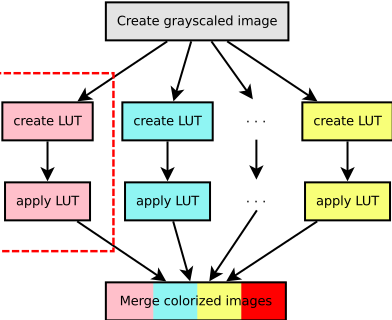
\includegraphics[width=0.75\textwidth]{fig/warholize-wkf2a}
\end{frame}


\begin{frame}
  \frametitle{The Warholize workflow, V}

  So, Step~2 is a \texttt{SequentialTaskCollection}-type task. Let's
  call this two-pass sequence \texttt{TricolorizeImage} .

  \+
  \includegraphics[width=0.75\textwidth]{fig/warholize-TricolorizeImage}
\end{frame}


\begin{frame}
  \frametitle{The Warholize workflow, VI}

  All the \texttt{TricolorizeImage} instances run in parallel. Collect
  them into a \texttt{ParallelTaskCollection}-type task, called
  \texttt{TricolorizeMultipleImages}.

  \+
  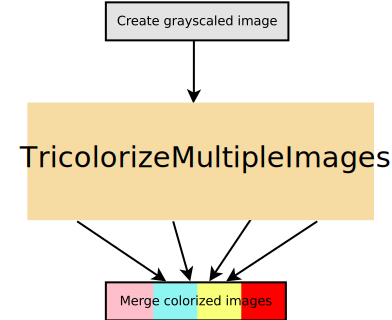
\includegraphics[width=0.75\textwidth]{fig/warholize-TricolorizeMultipleImages}
\end{frame}

\begin{frame}
  \frametitle{The Warholize workflow, VII}

  Now we are left with a three-step sequence: greyscale,
  \texttt{TricolorizeMultipleImages}, montage.  This can be defined
  again as a \texttt{SequentialTaskCollection}-type task, the
  \texttt{WarholizeWorkflow}.

  \+
  \includegraphics[width=0.70\textwidth]{fig/warholize-WarholizeWorkflow}
\end{frame}


\appendix

\end{document}

%%% Local Variables:
%%% mode: latex
%%% TeX-master: t
%%% End:
